\documentclass[a4paper]{article}
\usepackage[utf8]{inputenc} % Skal passe til editorens indstillinger
\usepackage[english]{babel} % danske overskrifter

\newcommand{\name}{Søren Krogh Andersen,\quad Carsten Nielsen}
\newcommand{\stnumber}{s123369,\quad s123161}
\newcommand{\course}{02155 Computer architecture}
\newcommand{\university}{Tehnical University of Denmark}
\newcommand{\studyline}{DTU Elektrotechnology}
\newcommand{\assignment}{Home Assignment 2}
\renewcommand{\date}{\today} %If another date, than that of today is desiered


% Palatino for rm and math | Helvetica for ss | Courier for tt
\usepackage{mathpazo} % math & rm
\linespread{1.05}        % Palatino needs more leading (space between lines)
\usepackage{palatino} % tt
\normalfont
\usepackage[T1]{fontenc}

\usepackage{graphicx}%allerese hentet % indsættelse af billeder
\usepackage{epstopdf} %Tilfj "--enable-write18" i argumentet for LaTex build. Dette vil konvertere .eps figurer til pdf-format
\graphicspath{{./picture/}} % stivej til bibliotek med figurer
\usepackage{subcaption} %Til gruppering af figurer
\usepackage{amsmath} %matpakke
\usepackage{amsfonts} %
\usepackage{amssymb} %
\usepackage{polynom} %for displaying polynom division
\usepackage{mathtools} % matematik - understøtter muligheden for at bruge \eqref{}
\usepackage{float}
\usepackage{hhline}
\usepackage[usenames,dvipsnames]{xcolor} %must be before loading other packages that use xcolor 
\usepackage{tikz}
\usepackage{pgfplots}
\usepackage{pgfplotstable}

%
\usepackage[compact,explicit]{titlesec}% http://ctan.org/pkg/titlesec
%

%Listings%
\usepackage{listingsutf8}
\usepackage{packs/mips}
%setup listings
\lstset{ %
  language=[mips]Assembler,       % the language of the code
  basicstyle=\footnotesize,       % the size of the fonts that are used for the code
  numbers=left,                   % where to put the line-numbers
  numberstyle=\tiny\color{gray},  % the style that is used for the line-numbers
  stepnumber=1,                   % the step between two line-numbers. If it's 1, each line 
                                  % will be numbered
  numbersep=5pt,                  % how far the line-numbers are from the code
  backgroundcolor=\color{white},  % choose the background color. You must add \usepackage{color}
  showspaces=false,               % show spaces adding particular underscores
  showstringspaces=false,         % underline spaces within strings
  showtabs=false,                 % show tabs within strings adding particular underscores
  frame=single,                   % adds a frame around the code
  rulecolor=\color{black},        % if not set, the frame-color may be changed on line-breaks within not-black text (e.g. commens (green here))
  tabsize=4,                      % sets default tabsize to 2 spaces
  captionpos=b,                   % sets the caption-position to bottom
  breaklines=true,                % sets automatic line breaking
  breakatwhitespace=false,        % sets if automatic breaks should only happen at whitespace
  title=\lstname,                 % show the filename of files included with \lstinputlisting;
                                  % also try caption instead of title
  keywordstyle=\color{blue},          % keyword style
  commentstyle=\color{Plum},       % comment style
  stringstyle=\color{mauve},         % string literal style
  escapeinside={\%*}{*)},            % if you want to add a comment within your code
  morekeywords={*,...}               % if you want to add more keywords to the set
}
 %Listings slut%









%"Matematik'' setioner
%\renewcommand\thesection{Question~\arabic{section}} %pas p�, kun i matematik
%\renewcommand\thesubsection{\thesection,~\alph{subsection}}
%\definecolor{MagRed}{RGB}{190,40,15}

%\titleformat{\section}{\normalfont\sffamily\large\bfseries\color{MagRed}}{}{0pt}{|\kern-0.15ex|\kern-0.15ex|\kern-0.15ex|~Question~\arabic{section}\qquad\quad#1\label{\arabic{section}}}
%\titleformat{\subsection}[runin]{\large\bfseries}{}{10pt}{\alph{subsection})~#1\label{\arabic{section}\alph{subsection}}}
%\titleformat{\subsubsection}[runin]{\itshape}{}{0pt}{~#1\label{\arabic{section}\alph{subsection}\arabic{subsubsection}}}
%\titleformat{\subsubsection}{\bfseries}{}{0pt}{\alph{subsection}.\arabic{subsubsection})\qquad\quad#1\label{\arabic{section}\alph{subsection}\arabic{subsubsection}}}



%Matematik hurtige ting
%fed
\renewcommand\vec[1]{\mathbf{#1}}
\newcommand\matr[3]{{}_{#2}\mathbf{#1}{}_{#3}}
\newcommand\facit[1]{\underline{\underline{#1}}}
%\renewcommand\d[3]{\frac{\mbox{d}^{#3}#1(#2)}{\mbox{d}#2^{#3}}}
%underline
%\renewcommand\vec[1]{\underline{#1}}
%\newcommand\matr[3]{{}_{#2}\underline{\underline{#1}}{}_{#3}}

\renewcommand\matrix[4]{ %{alignment}{to space}{from space}{matrix}
{\vphantom{\left[\begin{array}{#1}#4\end{array}\right]}}_{#2}\kern-0.5ex
\left[\begin{array}{#1}
#4
\end{array}\right]_{#3}
}
\newcommand\e[0]{\mbox{e}}
\newcommand\im[0]{i}

\newcommand\Jaco{\mbox{Jacobi}}
\newcommand\del[2]{\frac{\partial {#1}}{\partial {#2}}}
\newcommand\abs[1]{\left| {#1} \right|}
\newcommand\stdfig[4]{ %width,img,cap,lab
\begin{figure}[hb!]
\centering
\includegraphics[width={#1}\textwidth]{#2}
\caption{#3} \label{#4}
\end{figure}
}
\newcommand\diff{\dot}
\newcommand\ddiff{\ddot}


\textwidth = 400pt
\marginparwidth = 86pt
\hoffset = -25pt
\voffset= -10pt
\textheight = 630pt
\newcommand{\HRule}{\rule{\linewidth}{0.5mm}}
\usepackage{fancyhdr}
\usepackage[plainpages=false,pdfpagelabels,pageanchor=false]{hyperref} % aktive links
\hypersetup{%
  pdfauthor={\name - \stnumber},
  pdftitle={\assignment},
  pdfsubject={\course}}
%\usepackage{memhfixc}% rettelser til hyperref


\fancyhf{} % tom header/footer
\fancyhfoffset{20pt}
\fancyhfoffset{20pt}
\fancyhead[OL]{\name \\ \course}
\fancyhead[OC]{Date \\ \date}
\fancyhead[OR]{\university\\ \studyline}
\fancyfoot[FL]{}
\fancyfoot[FC]{\thepage}
\fancyfoot[FR]{}
\renewcommand{\headrulewidth}{0.4pt}
\renewcommand{\footrulewidth}{0.4pt}
\pagestyle{fancy}

% How to make ref to books or urls in bib
%\citetitle[fx: page 1]{name of ref in bib}

\begin{document}
\begin{titlepage}
\centering \parindent=0pt

\vspace*{\stretch{1}} \HRule\\[1cm]\Huge
\course\\[0.7cm]
\large \assignment\\[1cm]
\HRule\\[4cm]  
%\includegraphics[width=6cm]{picture}\\ Use this if you want a picture on the frontpage
\name\\
\stnumber

\vspace*{\stretch{2}} \normalsize %
\begin{flushleft}

\date \end{flushleft}
\vspace*{\stretch{2}} \normalsize
\begin{flushright}
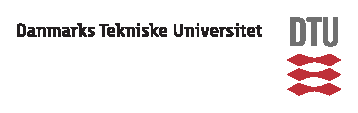
\includegraphics[width=6cm]{./DTU.eps}\\
\end{flushright}
\end{titlepage}


\begin{abstract}
This report will try to characterize how cacheparameters effect the sorting
algorithms \emph{bubblesort} and \emph{quicksort} on a single-cycle
\emph{MIPS-32} architecture.
Furtermore we will adapt the algorithms to handle records of variable size
(length and width) by sorting a list of only the record key and index of this
key, then arraning the record after these indexes.

Our findings are that both bubblesort and quicksort benefit from a large
blocksize, but if the blocksize is larger than twice the record width
(data-elements pr.\ record) a higher order of associativity is also needed.

The modified bubblesort benefits by a factor of $\sim10$ from the adapted
algorithm, while quicksort performs a bit slower.
\end{abstract}

\vspace{5cm}
Work Distribution
\begin{itemize}
	 \item Unoptimized Bubblesort and quicksort experiments: Carsten
	 \item Unoptimized Bubblesort and quicksort analysis: Carsten
	\item Modified bubblesort and quicksort analysis: Carsten
\end{itemize}

\newpage
\tableofcontents
\lstlistoflistings
\newpage
\section{Introduction}
In this report we will examine four programs. Two test programs that are designed to highlight specific cache behaviour and two
classic sorting algorithms, bubblesort and quicksort. The execution time of these programs is heavily dependent on cache parameters, 
such as block size, ways of associativity and total size. The programs are compiled for the MIPS architecture and executed on a 
single cycle MIPS-32 processor simulated by MipsIt. We will reason about the expected execution time of the programs as a function of
cache parameters, and compare our predictions to the measured statistics. We will also modify the classic algorithms to handle database
records, consisting of a key-value pair, sorting by the key and keeping the value unchanged. The performance of the modified programs 
will also be tested.

\section{Warm up}
\emph{test1.c} and \emph{test2.c} are two programs written to illustrate data
access and cache use. They both sum an array of $2048$ elements filled with ones
twice, with one of the summing runs ofsetted by the size of the cache. This is repeaded six
times. In both cases the result is $19200$.

\emph{test1.c} sums the elements like this:
\begin{lstlisting}
for ( j = 0; j < 5; j++ ) {
	sum += A[ i ];
	sum += A[ i + CACHE\_SIZE ];
}
\end{lstlisting}
ensuring that, atleast for a direct-mapped cache each access to the elements in
array $A$ is trashing the cache.

\emph{test2.c} sums first the lower half of the array (from $i=0$ to
$i=TAB_SIZE-CACHE\_SIZE-1$) six times, then the upper (from $i=CACHE\_SIZE$ to
$i=TAB_SIZE-1$).

\subsection{Initial remarks}
For all tests the instruction cache penalty has been turned off, so that this
does not affect test results.

In both \emph{test1.c} and \emph{test2.c} the \emph{promexit()} and
\emph{clear\_cache()} functions are put right after \emph{int main()}. This
ensures that the initialization of the processor (setting up stack and stuff we
don't have controll over) doesn't affect the profiling.

To test the program we run \emph{test.c} it with a cache size of $128$ words
arranged in blocks of $4$ on $32$ lines.

Running with a directmapped cache we expect the program to cache-trash all over
the place, and thus we expect a rather low hit rate. In the initalization we hit
on $\frac{3}{4}$ and miss on $\frac{1}{4}$ of the writes to $A$ - while during
the main data manipulation loop we miss on all accesses to $A$. Since this is
roughly 12 times as many misses - a hit rate in the area of $8\%$ is expected. 

Running the program, however, we get a hit rate of $84\%$! This requires an
explanation.
\subsubsection{Decompiling} and getting the assembler code, we can examine what
the compiler has done. In listing \ref{lst:test1ass} we have commented relevant
lines in the assembler code and noted which data accesses that are most likley
to be cache hits and misses:
\lstinputlisting[label={lst:test1ass}]{source/asm/test1.s}
It is clear that the ``problem'' is that $i$, $j$ and $sum$ are being read and
written to memory far more often than we access $A$.
Estimating the hit rate from the assembler code we get:

\begin{itemize}
  \item Hits:
  \begin{itemize}
    \item Initalization: For each loop, $i$ is accessed once for checking if the
    loop should continue, once to get the address of $A[i]$ and twice (r/w) for
    appending $i$.
    Due to the blocksize of 4, the write to $A[i]$ will be a hit
    $\frac{3}{4}$ of the time.
    \item Main data loop: $i$, $j$ and $sum$ are accessed $6\cdot 8 + 3$ times
    for each loop
  \end{itemize}
  \item Misses:
  \begin{itemize}
    \item Initalization: Due to the blocksize of 4, the write to $A[i]$ will be
    a miss $\frac{1}{4}$ of the time.
    \item Main data loop; $A[i]$ and $A[i + CACHE\_SIZE]$ will be misses and are
    accessed $6\cdot 2$ times for each loop.
  \end{itemize}
  \item hit rate can now be calculated as $\frac{\mbox{total
  hits}}{\mbox{total hits}+\mbox{total misses}}$ where $\mbox{total hits} =
  (4+3/4\cdot2048 + (6\cdot8+3)\cdot(2048-128))$ and $\mbox{total misses} =
  (1/4\cdot2048 + (6\cdot2)\cdot(2048-128))$. This gives a hit rate of $82\%$,
  not far from the actual hit rate.
\end{itemize}
\subsubsection{A note on \emph{mips.exe}} in the $D-cache$ window of mipset we
can get the actual total hits, misses, hit rate and execution clocks. These are, and
this is not a mistype, \emph{mips.exe} acually gives this data (our guess is
that mips forgot some zeroes, we have added those to the numbers in ``()''):
\begin{itemize}
  \item Hit count: $10516$ ($105160$)
  \item Miss count: $20282$ ($20282$)
  \item Hit rate: $0.84$ ($0.84$)
  \item Cycle count: $19205$ ($1920520$, from the data cache statistics)
\end{itemize}
this tells us that the total hitcount form the \emph{D-cache} window is not
reliable and cycle count should be taken from the data cache statistics window.

\subsubsection{Solution} digging arround on \emph{Stack Overflow} it turns out
the keyword \emph{register} tell the compiler to - if possible - store a variable in
registers. This keyword is put in front of $i$, $j$ and $sum$ as this makes it
possible to show the intended impact of different levels of associativity. With
the keyword in place we can now run \emph{test1.c} and \emph{test2.c} and give
meaningfull explanations to why the hit rate is affected as it is. Furthermore
as optimization level will be increased to $2$ for the sorting algorithms - this
will make the compiler use registers for variables for the rest of the
assignment too.

\subsection{Test results for test1 and test2 with varying level of
associativity}
\emph{test1.c} and \emph{test2.c} are run with and without the register keyword
and with associativity 1, 2, 4 and 8. We note for both tests without the
register keyword that their hit rate is extremly high - while the cycle count is
the higest too. This is because the general use of memory operations is
significantly lager too.

\begin{table}[H]
  \centering
  \begin{tabular}{c | c | c | c |}
    Test	&	Blocks in set	&	Cycle count	&	Hit rate	\\ \hline
    Test1 vars not in regs
    		&	1				&	1920520		&	84\%		\\ \hline
    Test2 vars not in regs
    		&	1				&	1364463		&	98\%		\\ \hline \hline
    %
    Test1	&	1				&	1264021		&	9\%			\\ \hline
    Test1	&	2				&	367073		&	91\%		\\ \hline
    Test1	&	4				&	343569		&	93\%		\\ \hline
    Test1	&	8				&	339045		&	93\%		\\ \hline \hline
    %
    Test2	&	1				&	398520		&	93\%		\\ \hline
    Test2	&	2				&	398520		&	93\%		\\ \hline
    Test2	&	4				&	398520		&	93\%		\\ \hline
    Test2	&	8				&	398520		&	93\%		\\ \hline 
  \end{tabular}
  \caption{Test results for test1 and test2}
  \label{tab:test}
\end{table}

\subsubsection{Conclution based on data in figure \ref{tab:test}, test1}
For test1 we get a low hit rate (and slow execution time) for the directmapped
cache we have a hit rate of $9\%$. We, however, gain a good speedup, when using
a two-way associative cache - this allows both $A[i]$ and $A[i + CACHE\_SIZE]$
to be kept in cache. Inceasing the associativity from here doesn't really do
much, we already hit on $\frac{10}{12}$ memory accesses. We gain a bit from
reusing the $x + CACHE\_SIZE$'th element when $i = x + CACHE\_SIZE$ so that an
ealier cached $A[x + CACHE\_SIZE] = A[i]$.

\subsubsection{Conclution based on data in figure \ref{tab:test}, test2}
Increasing the associativity for test2 has litte to no influence. Test2 performs
well for a directmapped cache, compared to test1 - as we are not accessing
elements that are spaced by the $CACHE\_SIZE$ directly after eachother. For
higher levels of associativity we gain no increased performance - this is
because the chance of element $A[i]$ to still be in the cache, when it is needed
for the second run throug the array is insignificantly small (for a two-way
associative cache elemet $A[i]$ has a chance of still being in the cache, when
it has to be used again is $\frac{1}{2}^\frac{1920}{64}$).

Since test2 has to run through the loop twice, for a cache with associativity
over $1$ test1 is actually faster in these cases.

\section{Bubblesort and quicksort}

\subsection{Bubblesort}
The bubblesort algorithm given in the exercise manual contains two bugs. It will not sort the first element of a given list and the 
outer loop goes out of bounds. The algorithm also needs to be modified to sort both the record keys and values. 
The fixed code is shown in listing~\ref{bubblesort1list} together with the main function that executes the test.
Since arrays in C are organized in row-major order, it is expected that the bubblesort algoritm will benefit greatly from increased
block size in the cache. This is due to the fact that bubblesort, for a record length of seven, compares elements in memory with a 
stride of 7, and accesses all elements between the first element accessed and \(2*RECORD\_LENGTH\) on a swap. Thus, for the naive
bubblesort, increasing block size should always improve performance. The bubblesort algorithm shown in the listing above, however, 
exploits the fact that the largest element will always be correctly placed after the first iteration, the second largest element
after the second iteration and so forth. This places an upper bound on the effectiveness of increasing block size as unused words
will needlessly be loaded and replaced in the cache. If associativity is increased, this upper bound should move back
further since large blocks will be able to coexist in the same set. Thus removing the penalty for accessing only a few 
elements, that map to the same block, outside of a large block.

\subsubsection{Bubblesort test}
Testing bubblesorts dependency on cache parameters was done by running the bubblesort test program for all power of two combinationes
of block sizes 1-64 words and 1-4 blocks per set, as associativity greater than 4 barely decreases miss rate \cite[p.~484]{HandP}.
The total cache size was kept constant at 512 words.

\begin{figure}[H]
	\flushleft
	\begin{minipage}[c]{0.4\textwidth}
		\scalebox{0.5}{
			\begin{tabular}{c | r | r | r }
				Block size / words & Blocks per set & hit \% & Execution time / ns \\ \hline
				1& 1& 78& 425391272 \\ \hline
				1& 2& 78& 413453090 \\ \hline
				1& 4& 78& 412887614 \\ \hline  
				2& 1& 88& 235780820 \\ \hline
				2& 2& 88& 232451104 \\ \hline
				2& 4& 88& 231967648 \\ \hline
				4& 1& 92& 140191677 \\ \hline
				4& 2& 92& 134672553 \\ \hline
				4& 4& 93& 134200693 \\ \hline
				8& 1& 94&  99320731 \\ \hline
				8& 2& 96&  88988171 \\ \hline
				8& 4& 96&  88561691 \\ \hline
				16&1& 95&  81937382 \\ \hline
				16&2& 98&  63179822 \\ \hline
				16&4& 98&  62679254  \\ \hline
				32&1& 94& 103627999 \\ \hline
				32&2& 99&  54189887  \\ \hline
				32&4& 99&  53796655 \\ \hline
				64&1& 91& 167612952 \\ \hline
				64&2& 99&  45967056 \\ \hline
				64&4& 99&  45382728 \\ \hline
		\end{tabular} }
	\end{minipage}
	\begin{minipage}[c]{0.4\textwidth}
		\begin{tikzpicture}
			\begin{loglogaxis}[log basis x=2, log basis y=2, xlabel=Block size / words, ylabel=Blocks per set, zlabel=execution time / ns,
					xtick={1,2,4,8,16,32,64},
					ytick={1,2,4},
					view = {120}{35},% important to draw x,y in increasing order
					xmin = 0,
					ymin = 0,
					xmax = 128,
					ymax = 8,
					zmin = 0,
					unbounded coords = jump,
					colormap={pos}{color(0cm)=(white); color(6cm)=(orange)}
				]
				\addplot3[surf,mark=none, shader=flat, draw=mapped color!80!black] file {source/python/bubblesort.dat};

			\end{loglogaxis}
		\end{tikzpicture}
	\end{minipage}
	\caption{Test results for bubblesort with a cache size of 512 words.}
	\label{fig:bubbleResults}
\end{figure}
The test results can be seen in figure (~\ref{fig:bubbleResults}).

From the results we can see that the maximum blocksize for a directmapped cache, before execution time starts rising again, is 
16 words. This is just as expected, as the record size the algorithm is working on contains records of size 7.
Thus there is a high probability that a swap sequence will have all the elements to be swapped already in cache,
because the preceding compare action already brought them in.

\subsection{Quicksort}
The quicksort algorithm given in the exercise manual does not contain any bugs, but needs to be modified to handle records instead
of single integers. The modified algorithm is shown in listing~\ref{quicksort1list}.
For quicksort we do not expect the same dependency on cache parameters as for bubblesort. This is due to quicksort not 
having the same spatial locality as bubblesort, since quicksort compares elements on opposite sides of a certain point. 
The record sorting quicksort will however benefit from increased block size as less cache misses will occur when swapping if
more elements of a single record are brought into cache, when attempting to access the record key for comparison. Associativity is
not expected to greatly affect the execution time unless the block size is large. This is again due to the loading/eviction of 
unnecessary elements.

\subsubsection{Quicksort test}
Quicksort was tested for the same cache parameters as bubblesort. The results can be seen in figure (~\ref{fig:quickResults}).
\begin{figure}[H]
	\flushleft
	\begin{minipage}[c]{0.4\textwidth}
		\scalebox{0.5}{
			\begin{tabular}{c | r | r | r }
				Block size / words & Blocks per set & hit \% & Execution time / ns \\ \hline
				 1& 1& 74&   3431095 \\ \hline
				 1& 2& 74&	 3451395 \\ \hline
				 1& 4& 73&   3478195 \\ \hline
				 2& 1& 84&   2075397 \\ \hline
				 2& 2& 84&   2077737 \\ \hline
				 2& 4& 94&   2090477 \\ \hline
				 4& 1& 88&   1361177 \\ \hline
				 4& 2& 89&   1354573 \\ \hline
				 4& 4& 88&   1358421 \\ \hline
				 8& 1& 92&   1004953 \\ \hline
				 8& 2& 92&    994313 \\ \hline
				 8& 4& 92&    997337 \\ \hline
				 16&1& 95&    752365 \\ \hline
				 16&2& 96&    709037 \\ \hline
				 16&4& 96&    708525 \\ \hline
				 32&1& 96&    753393 \\ \hline
				 32&2& 98&    623945 \\ \hline
				 32&4& 98&    622065 \\ \hline
				 64&1& 95&    937653 \\ \hline
				 64&2& 99&    545204 \\ \hline
				 64&4& 99&    537269 \\ \hline
		\end{tabular} }
	\end{minipage}
	\begin{minipage}[c]{0.4\textwidth}
		\begin{tikzpicture}
			\begin{loglogaxis}[log basis x=2, log basis y=2, xlabel=Block size / words, ylabel=Blocks per set, zlabel=execution time / ns,
					xtick={1,2,4,8,16,32,64},
					ytick={1,2,4},
					view = {120}{35},% important to draw x,y in increasing order
					xmin = 0,
					ymin = 0,
					xmax = 128,
					ymax = 8,
					zmin = 0,
					unbounded coords = jump,
					colormap={pos}{color(0cm)=(white); color(6cm)=(orange)}
				]
				\addplot3[surf,mark=none, shader=flat, draw=mapped color!80!black] file {source/python/quicksort.dat};

			\end{loglogaxis}
		\end{tikzpicture}
	\end{minipage}
	\caption{Test results for quicksort with a cache size of 512 words.}
	\label{fig:quickResults}
\end{figure}
At first glance these results seem very similar to those obtained for the bubblesort algorithm except for the fact that quicksort is 
two orders of magnitude faster. Even though there is a significant performance gain when increasing block size, it can be seen that 
quicksort has less relative performance gain from increased block size than bubblesort, as
predicted. The large performance gain is the result of having a higher probability of not incurring a cache miss when swapping records
when the block size is appropriately large. 
Also, the performance gain from increased associativity is negligible except for block sizes of 32 words or larger.

\section{Handling variable record sizes and optimizing bubblesort and quicksort}
One apparent problem with the algorithms used in the previous section is the amount of needless swapping taking place, more so
for bubblesort than quicksort. To solve this problem we have modified the algorithms to start by creating a new array, copying 
the record keys and their index in the original array. Then this array is sorted according to keys and the index is used to copy 
records from the original array and then restore them in the original array in the correct positions. If the sorted data does not have
to be in the same memory location after the sorting, it is possible to reduce the runtime significantly by simply pointing to the newly
created array. However, we assume that the data must stay sorted in the original location.

The modified code can also handle records of variable length, defined at runtime, but the variable length is managed by \#defines
in the test code for simplicity. Our test code is shown below
\lstinputlisting[language=C, caption=Test code for the variable record length versions of quicksort and bubblesort]{source/c/quicksort_n.c}
\subsection{Test results}
The test of the variable record length versions of quicksort and bubblesort was performed in the same way as the fixed record length ones.
\subsubsection{Bubblesort}
The test results for the variable record length bubblesort can be seen in figure (~\ref{fig:bubbleVarResults})
\begin{figure}[H]
	\flushleft
	\begin{minipage}[c]{0.4\textwidth}
		\scalebox{0.5}{
			\begin{tabular}{c | r | r | r }
				Block size / words & Blocks per set & hit \% & Execution time / ns \\ \hline
				1& 1& 55& 29344780 \\ \hline
				1& 2& 57& 28348585 \\ \hline
				1& 4& 57& 27946935 \\ \hline  
				2& 1& 58& 29083395 \\ \hline
				2& 2& 59& 28045527 \\ \hline
				2& 4& 59& 27629527 \\ \hline
				4& 1& 78& 17146977 \\ \hline
				4& 2& 78& 16626613 \\ \hline
				4& 4& 79& 16419809 \\ \hline
				8& 1& 89& 11638889 \\ \hline
				8& 2& 89& 11354073 \\ \hline
				8& 4& 90& 11239161 \\ \hline
				16&1& 95& 8873675 \\ \hline
				16&2& 95& 8706443 \\ \hline
				16&4& 95& 8643555  \\ \hline
				32&1& 97& 7988865 \\ \hline
				32&2& 97& 7842091  \\ \hline
				32&4& 97& 7791009 \\ \hline
				64&1& 99& 7140151\\ \hline
				64&2& 99& 7005623 \\ \hline
				64&4& 99& 6953655 \\ \hline
		\end{tabular} }
	\end{minipage}
	\begin{minipage}[c]{0.4\textwidth}
		\begin{tikzpicture}
			\begin{loglogaxis}[log basis x=2, log basis y=2, xlabel=Block size / words, ylabel=Blocks per set, zlabel=execution time / ns,
					xtick={1,2,4,8,16,32,64},
					ytick={1,2,4},
					view = {120}{35},% important to draw x,y in increasing order
					xmin = 0,
					ymin = 0,
					xmax = 128,
					ymax = 8,
					zmin = 0,
					unbounded coords = jump,
					colormap={pos}{color(0cm)=(white); color(6cm)=(orange)}
				]
				\addplot3[surf,mark=none, shader=flat, draw=mapped color!80!black] file {source/python/bubblesort_n.dat};

			\end{loglogaxis}
		\end{tikzpicture}
	\end{minipage}
	\caption{Test results for variable record length bubblesort with a cache size of 512 words.}
	\label{fig:bubbleVarResults}
\end{figure}
From the test results we can conclude that the modified bubblesort is much faster than the original by approximately a factor of 10.
The hit rate is much lower than the original bubblesort for small block sizes. This is a result of the large amount of copying taking
place when the algorithm is about to complete. The actual sorting part of the algorithm has a hit rate in the 90th percentile. It 
can also be seen that there is no significant difference in execution time for block sizes 1 and 2. This is because the array being
sorted always accesses memory with a stride of 2 when comparing. Thus a miss will always happen on comparison for these block sizes.
Furthermore we note that the associativity level does not affect the execution time like it did for the original bubblesort. 
This is due to the nature of bubblesort. Since the algorithm always compares elements that are next to each other, eviction of 
elements that will be needed in the near future is very rare. The original bubblesort showed a performance gain from increased 
associativity for large block sizes which can be explained by the higher probability that an element in the record would cross a
block boundary and thus initiate an entire block transfer, since the entire record was swapped.

\subsubsection{Quicksort}
\begin{figure}[H]
	\flushleft
	\begin{minipage}[c]{0.4\textwidth}
		\scalebox{0.5}{
			\begin{tabular}{c | r | r | r }
				Block size / words & Blocks per set & hit \% & Execution time / ns \\ \hline
				1& 1& 55& 29344780 \\ \hline
				1& 2& 57& 28348585 \\ \hline
				1& 4& 57& 27946935 \\ \hline  
				2& 1& 58& 29083395 \\ \hline
				2& 2& 59& 28045527 \\ \hline
				2& 4& 59& 27629527 \\ \hline
				4& 1& 78& 17146977 \\ \hline
				4& 2& 78& 16626613 \\ \hline
				4& 4& 79& 16419809 \\ \hline
				8& 1& 89& 11638889 \\ \hline
				8& 2& 89& 11354073 \\ \hline
				8& 4& 90& 11239161 \\ \hline
				16&1& 95& 8873675 \\ \hline
				16&2& 95& 8706443 \\ \hline
				16&4& 95& 8643555  \\ \hline
				32&1& 97& 7988865 \\ \hline
				32&2& 97& 7842091  \\ \hline
				32&4& 97& 7791009 \\ \hline
				64&1& 99& 7140151\\ \hline
				64&2& 99& 7005623 \\ \hline
				64&4& 99& 6953655 \\ \hline
		\end{tabular} }
	\end{minipage}
	\begin{minipage}[c]{0.4\textwidth}
		\begin{tikzpicture}
			\begin{loglogaxis}[log basis x=2, log basis y=2, xlabel=Block size / words, ylabel=Blocks per set, zlabel=execution time / ns,
					xtick={1,2,4,8,16,32,64},
					ytick={1,2,4},
					view = {120}{35},% important to draw x,y in increasing order
					xmin = 0,
					ymin = 0,
					xmax = 128,
					ymax = 8,
					zmin = 0,
					unbounded coords = jump,
					colormap={pos}{color(0cm)=(white); color(6cm)=(orange)}
				]
				\addplot3[surf,mark=none, shader=flat, draw=mapped color!80!black] file {source/python/quicksort_n.dat};

			\end{loglogaxis}
		\end{tikzpicture}
	\end{minipage}
	\caption{Test results for variable record length quick with a cache size of 512 words.}
	\label{fig:quickVarResults}
\end{figure}

\section{Conclusion}
The orignal bubblesort and quicksort algorithms depend heavily upon cache parameters for optimizing execution time. 
Their respective execution times both reached a minimum value for a directmapped cache when two records could fit in a single block.
We did not find an upper bound on the effectiveness of increasing block size when the cache also had more ways of associativity. However,
it was observed that increasing associativity and block size yielded diminishing returns.

The modified algorithms that handle variable length records also tried reducing the execution time by sorting smaller memory chunks.
This proved immensely effective for bubblesort, reducing the execution time by more than a factor of 10, but failed for quicksort. It 
was observed that the execution time of the modified quicksort approached the original as the record size increased and so there is 
reason to believe that it will be faster for very large record sizes. However, it did not
perform better for record sizes in the interval 3-64 that were specified in the exercise manual.

\appendix
\section{Code listings}
\lstinputlisting[label={lst:test1ass}, label=test1ass,
caption={Assemblycode for \emph{test1.c} with our comments
added (the ``sp not trusted'' is not from us)}]{source/asm/test1.s}
\lstinputlisting[language=C, label=bubble1list,caption=Bubblesort test program]{source/c/bubblesort.c}
\lstinputlisting[language=C, label=quicksort1list, caption=Quicksort test program]{source/c/quicksort.c}
\lstinputlisting[language=C,label=varlist, caption=Test code for the variable record length versions of quicksort and bubblesort]{source/c/quicksort_n.c}


\begin{thebibliography}{9}

\bibitem{HandP}
  David A. Patterson and John L. Hennessy,
  \emph{Computer Organization and Design, the software / hardware interface}.
  Morgan Kaufmann,
  4th Edition revised printing,
  2012.
\bibitem{StackRegPost}
  Various,
  \url{http://stackoverflow.com/questions/15908835/c-c-register-variable}
  Internet forum,
  4/12-2013.

\end{thebibliography}
\end{document}
